\section{Arithmetic prediction and homological consequences}\label{sec:prediction}
\subsection{What arithmetic predicts}
Paper~III proves that the step at which the occurrence set next changes is given by a congruence sieve: with $Y_j=ah+jL^2$ the integers $d\ge2$ occur at the stage $j$ iff $Q(d)\mid Y_j$ (\Src{III}{thm:sieve}), so the event time is computed from divisibility alone (\Src{III}{cor:event}); and that the first occurrences that arrive in an activation family are determined by explicit moduli (\Src{III}{thm:A5T24}). The homological consequences are governed by the zig-zag identity $K\leftarrow K^\circ\to K'$ (\Src{III}{thm:zigzag}) and, for nested events, $\Delta\beta_i=h_i(K',K)-k_i-k_{i-1}$ (\Src{III}{thm:nested}). The question is how much of $\Delta\beta$ is determined by cheaper data.

\noindent\Cref{fig:event} shows arithmetic prediction of collective occurrence events.

\begin{figure}[t]\centering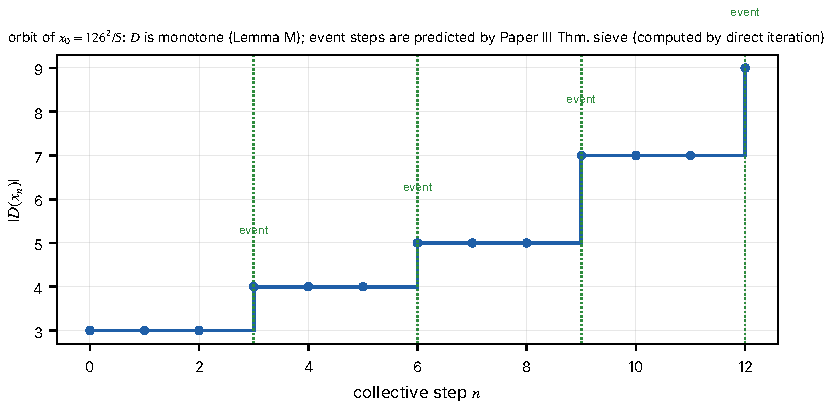
\includegraphics[width=\linewidth]{fig13_event_prediction.pdf}
\caption{\textbf{Arithmetic prediction of collective occurrence events.} The size $|D(x_n)|$ along the orbit of $126^2/5$: monotone with events at the steps predicted by the stage sieve (\Src{III}{thm:sieve}). \emph{The mechanism is the cited theorem; the plotted values are computed by direct iteration.}}\label{fig:event}\end{figure}
\subsection{Information requirements}
\begin{proposition}[\SIV{7}: information requirements for topological prediction]\label{prop:P7}\status{new, proved; witnesses finite-exact}
Let $D\subseteq D'=D\cup N$ be finite sets of integers $\ge2$ (statements (a)--(d) concern the abstract complexes $K(D),K(D')$; the witnesses of (d) are abstract and are not claimed to occur along collective orbits) with $K=K(D)$, $K'=K(D')$, local data $\lambda=(f(K),f(K'),\text{dead cells},\text{new cells})$, where $f$ is the cell-count vector.
\begin{enumerate}[label=(\alph*),itemsep=1pt]
\item \emph{Euler.} $\sum_i(-1)^i\Delta\beta_i=\sum_i(-1)^i\Delta f_i$; the right side is a function of $\lambda$.
\item \emph{First Betti number from supports.} $\Delta\beta_0=\mathrm{cl}(D')-\mathrm{cl}(D)$ where $\mathrm{cl}$ is the number of classes of the share-a-prime relation (\cref{lem:comp}); it is a function of the prime supports of $D$ and $N$ and does not need the complexes.
\item \emph{Graph level is determined.} If $K$ and $K'$ have no $2$-cells, then $\Delta\beta_1=\Delta f_1-\Delta f_0+\Delta\beta_0$ and $\Delta\beta_i=0$ for $i\ge2$. Thus $(\lambda,\text{supports})$ determine $\Delta\beta$ completely.
\item \emph{Obstruction: $\lambda$ alone does not determine $\Delta\beta$ (abstract set-level events).} The events $D=\{385,27720\}$, $N=\{11,72\}$ and $D=\{15,315\}$, $N=\{4,21\}$ have the same $\lambda$ ($f=(2,1,0)\to(4,3,0)$, nothing lost, $2$ new vertices and $2$ new edges), with $\Delta\beta=(0,0,0)$ and $(+1,+1,0)$. Likewise $D=\{12,35\},N=\{44,45\}$ and $D=\{33,280\},N=\{14,20\}$ have $f=(2,0,0)\to(4,3,0)$ and $\Delta\beta=(-1,0,0)$ versus $(0,+1,0)$.
\item \emph{Beyond graph level (open).} When $2$-cells are present, $\lambda$ together with $\Delta\beta_0$ fixes only the alternating sum $\Delta\beta_1-\Delta\beta_2+\cdots$. We know of no pair with equal $\lambda$ and equal $\Delta\beta_0$ but different $(\Delta\beta_1,\Delta\beta_2)$: a random search of $60{,}000$ events ($2{,}039$ distinct values of $(\lambda,\Delta\beta_0)$ with $2$-cells) found none. This is not a theorem (O4).
\end{enumerate}
\end{proposition}
\begin{proof}
(a) For finite complexes $\chi=\sum(-1)^i\beta_i=\sum(-1)^if_i$ over any field. (b) is \cref{lem:comp} applied to $D$ and $D'$. (c) By (a) with $f_i=0$ for $i\ge2$: $\Delta\beta_0-\Delta\beta_1=\Delta f_0-\Delta f_1$, and higher Betti numbers vanish for a graph. (d) The values of $\lambda$ and the Betti numbers of the four complexes are recomputed with the exact engine (Appendix~\ref{app:obstructions}, E5); they also illustrate (b) and (c): in the first pair $\Delta f_1-\Delta f_0=0$, so $\Delta\beta_1=\Delta\beta_0$, which is $0$ for $\mathrm{cl}:1\to1$ and $+1$ for $\mathrm{cl}:1\to2$; in the second pair $\Delta f_1-\Delta f_0=+1$ and $\mathrm{cl}:2\to1$, $2\to2$ give $\Delta\beta_1=0$ and $+1$. (e) records a search outcome.
\end{proof}
\begin{remark}
The arithmetic therefore predicts \emph{when} the occurrence set changes (sieve) and \emph{what} $\beta_0$ and, at graph level, $\beta_1$ become (supports and local counts). What is not predicted from local counts is how new cells attach to old homology classes in positive degree; that information is the attachment data $(r_i,h_i,\beta(K^\circ))$ of \Src{III}{thm:zigzag}.
\end{remark}

\noindent\Cref{fig:local} shows surviving complex and homological attachment information.

\begin{figure}[t]\centering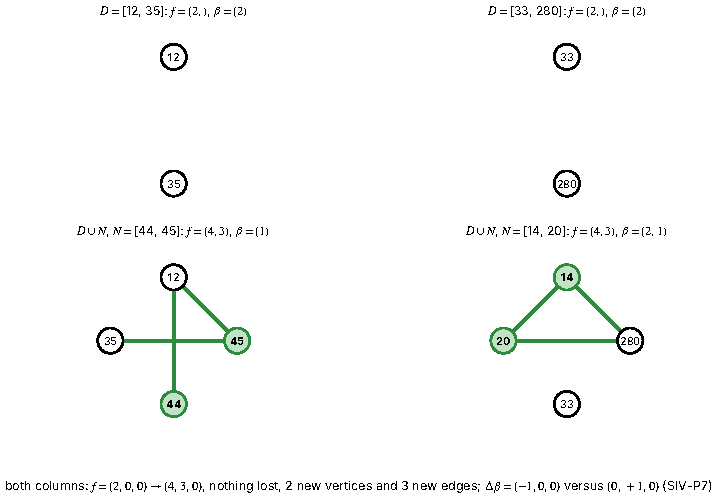
\includegraphics[width=\linewidth]{fig17_local_inventory.pdf}
\caption{\textbf{Surviving complex and homological attachment information.} Two events with identical local counts $f=(2,0,0)\to(4,3,0)$ and different Betti changes: $\Delta\beta=(-1,0,0)$ and $(0,+1,0)$. The difference is carried by the prime supports of the new vertices relative to the old components (\cref{prop:P7}(b),(c)). \emph{Exact.}}\label{fig:local}\end{figure}
